\chapter{Part II(d) - Processor, I/Os, and Exceptions}

\section{Exceptions, Interrupts, Faults, Traps, and Checks}

\paragraph{Control Flow}
Under normal circumstances, the \textit{control flow}—the sequence of instructions executed by a program—is fully determined by the programmer. This includes the use of jumps, branches, and procedure calls.

\paragraph{Exceptions}
Exceptions represent a deviation from the normal control flow. They are triggered by \textbf{special conditions} that are not explicitly defined in the program. When an exception occurs, the control flow changes unexpectedly, and the program must respond accordingly.

\paragraph{Exception Handlers}
To manage exceptions, \textit{exception handlers} are invoked. These are specialized functions designed to take appropriate actions when an exception arises. An example of this is \textbf{I/O interrupts}, which signal specific events related to input/output operations.

\paragraph{Naming Conventions}
The terminology for exceptions and related events varies widely across systems. For clarity, we adopt the following convention based on RISC-V and the COD:
\begin{itemize}
    \item \textbf{Exceptions:} A general term encompassing all control flow deviations.
    \item \textbf{Interrupts:} A specific type of exception generated outside the processor.
\end{itemize}
Thus far, interrupts are the only form of exception encountered.

\subsection{Undefined Instruction}

Undefined instructions are instructions that the controller does not recognize, as they do not correspond to any valid operation in the Instruction Register (IR). These scenarios require special handling to ensure system stability and proper exception processing.

\vspace{0.5cm}
\begin{minipage}[htp]{0.35\textwidth}
- \textbf{Detection:} When an undefined instruction is detected in the IR, the controller generates a signal (\texttt{undef}) indicating the presence of an invalid operation. \\ 
- \textbf{Exception Handling:} The Program Counter (PC) is updated to the address of the Exception Handler to manage the undefined instruction. This involves: \\
\begin{itemize}
\item Saving the current PC for potential recovery.
\item Redirecting the control flow to the exception handler's address using multiplexer logic.
\end{itemize}
- \textbf{Control Logic:} The system leverages the Next PC Logic to determine whether the next instruction comes from the regular PC logic or the exception handler, based on the \texttt{undef} signal or an external interrupt (IRQ).
\end{minipage}
\hfill
\vline
\hfill
\begin{minipage}[htp]{0.55\textwidth}
    \begin{center}
        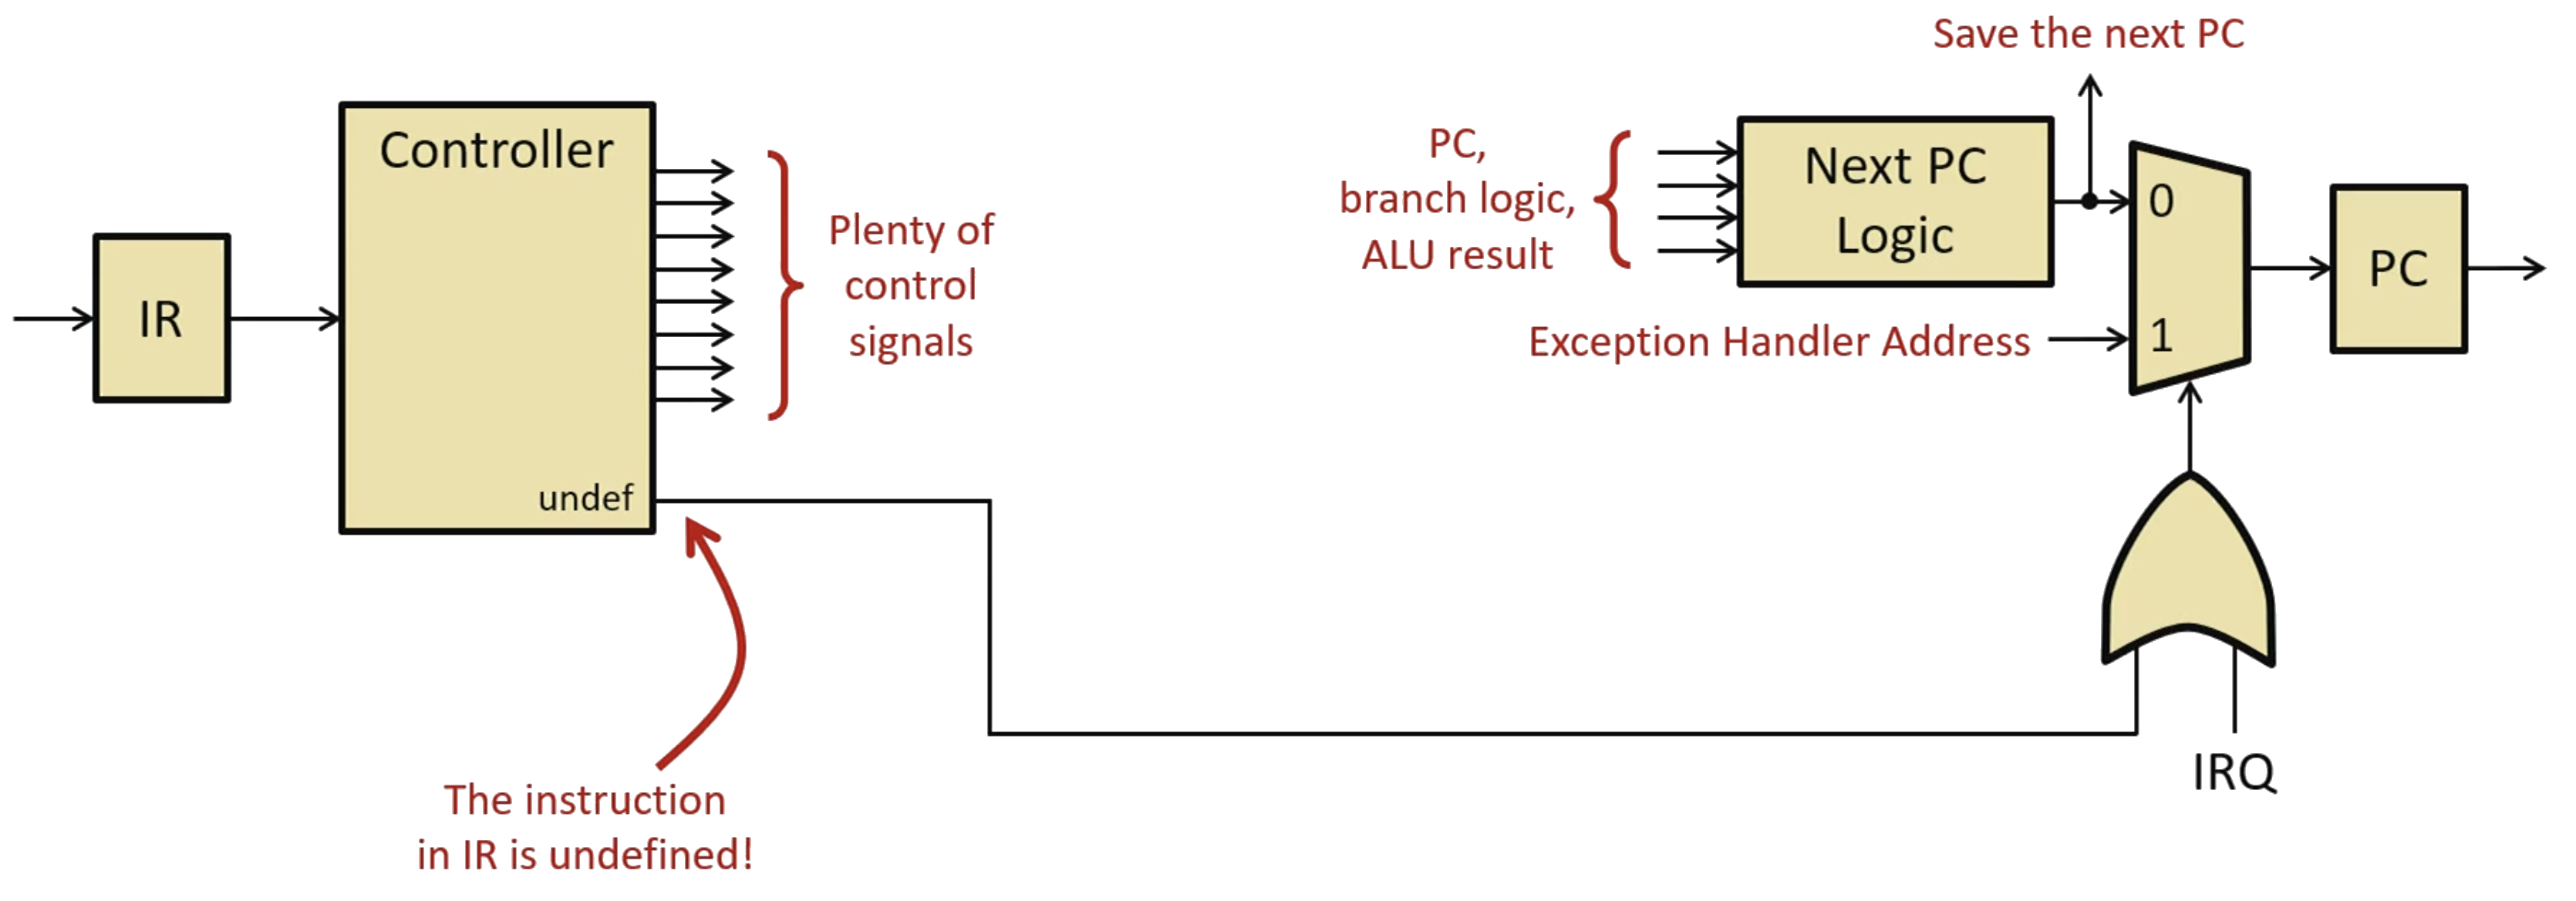
\includegraphics[width=1.2\textwidth]{chapters/chapter2d/images/undefined.png}
    \end{center}
\end{minipage} \\
\vspace{0.5cm}
- \textbf{Synchronous Nature:} These exceptions occur at a specific point in the program, precisely where the undefined instruction resides. This predictable behavior ensures that if the program is re-executed from the same initial state, the exception will occur at the exact same point, making debugging more straightforward. \\ \vspace{0.5cm}
- \textbf{Immediate Handling:} Serving the exception before executing the next instruction allows advanced features, such as efficient error recovery and the potential to extend system capabilities.
\vspace{0.5cm}
This mechanism ensures that undefined instructions do not disrupt the execution flow and are handled systematically, enabling robust error recovery and system stability.

\subsection{Optional \texttt{fadd.s} Instruction}

Suppose we want to include a floating-point addition instruction, denoted as:
\begin{assembly}
fadd.s rd, rs1, rs2
\end{assembly}

- Some processors might include a specialized ALU to support this instruction, whereas \textbf{cheaper processors do not}. \\ \vspace{7px}
- For processors that lack support for this instruction, its execution would trigger an \textit{undefined instruction exception}, which invokes a handler. \\ \vspace{7px}
- The handler can \textbf{emulate} the behavior of the \texttt{fadd.s} instruction, ensuring compatibility across processors. \\ \vspace{7px}

\subsection{Outline of an Undefined Instruction Handler}
To handle an undefined instruction, such as \texttt{fadd.s}, the following steps wouls be executed:
\begin{itemize}
    \item[] \textbf{Save all registers} on the stack that the handler or its callees might modify.
    \begin{itemize}
        \item Note: Standard calling conventions do not apply.
    \end{itemize}
    \item[] \textbf{Retrieve the problematic instruction}:
    \begin{itemize}
        \item If the program counter (PC) is saved, load the instruction from the corresponding address.
    \end{itemize}
    \item[] \textbf{Decode the instruction} in software and identify it as \texttt{fadd.s}.
    \item[] \textbf{Read the source registers} (operands) and either:
    \begin{itemize}
        \item Call a library function, or
        \item Implement the floating-point addition in software.
    \end{itemize}
    \item[] \textbf{Store the result} in the destination register.
    \item[] \textbf{Update the program counter (PC)} to point to the next instruction.
    \item[] \textbf{Jump to the updated PC} to resume execution.
\end{itemize}

\section{Exceptions and Interrupts}
Exceptions, interrupts, and related mechanisms handle critical events during execution. Key use cases include:
\begin{itemize}
    \item[] \textbf{I/O Requests:} Processing data or new inputs.
    \item[] \textbf{Timer Interrupts:} Handling time-based events.
    \item[] \textbf{Undefined Instructions:} E.g., unsupported floating-point operations.
    \item[] \textbf{Arithmetic Faults:} Errors like division by zero.
    \item[] \textbf{Memory Violations:} Unauthorized access to restricted memory.
    \item[] \textbf{Debugging:} Breakpoints and execution control.
    \item[] \textbf{Hardware Failures:} Malfunctions such as power loss.
\end{itemize}
\subsection{A Possible Classification of Exceptions}
\begin{center}
    \begin{tabular}{|l|l|l|l|}
    \hline
    \textbf{Type}                     & \textbf{Synchronous?} & \textbf{Coerced?}      & \textbf{Resume?} \\ \hline
    I/O request                       & Asynchronous          & Coerced               & Resume           \\ \hline
    Invoke OS                         & Synchronous           & User requested        & Resume           \\ \hline
    Trace instruction                 & Synchronous           & User requested        & Resume           \\ \hline
    Breakpoint                        & Synchronous           & User requested        & Resume           \\ \hline
    Page fault                        & Synchronous           & Coerced               & Resume           \\ \hline
    Misaligned access                 & Synchronous           & Coerced               & Resume           \\ \hline
    Memory protection violation       & Synchronous           & Coerced               & Terminate        \\ \hline
    Bus error                         & Synchronous           & Coerced               & Terminate        \\ \hline
    Arithmetic fault                  & Synchronous           & Coerced               & Terminate        \\ \hline
    Undefined instruction             & Synchronous           & Coerced               & Terminate        \\ \hline
    Hardware malfunction              & Asynchronous          & Coerced               & Terminate        \\ \hline
    Power failure                     & Asynchronous          & Coerced               & Terminate        \\ \hline
    \end{tabular}
\end{center}

\begin{itemize}
    \item \textbf{Synchronous?} Indicates whether the exception occurs as a direct result of the execution flow (synchronous) or independently of it (asynchronous).
    \item \textbf{Coerced?} Specifies whether the exception is forced by the system (coerced) or triggered by a user request.
    \item \textbf{Resume?} Denotes whether the system can continue executing after handling the exception (resume) or must terminate.
\end{itemize}